\chapter{Activation Records}
Er is een overstap nodig naar een neutrale voorstelling die onafhankelijk is van de oorspronkelijke taal. Er is wel een probleem: zelfs de omzetting van de abstract syntax tree naar deze neutrale voorstelling is afhankelijk van de architectuur waarvoor gecompileerd wordt. Bijvoorbeeld het statement \texttt{*p++} in C is anders voor 32-bit of 64-bit systemen. Het doel is om de taalspecifieke Abstract Syntax Tree om te vormen naar een taalonafhankelijke Intermediate Representation Tree.

Bij de meeste talen worden er lokale variabelen gecreëerd bij het aanroepen van een functie. Meerdere instanties van een functie kunnen bestaan en hebben elk hun eigen instanties van lokale variabelen.
\begin{lstlisting}
function f(x: int) : int =
  let var y := x + x
   in if y < 10
          then f(y)
          else y - 1
end
\end{lstlisting}
Een instantie van $x$ wordt aangemaakt elke keer dat $f$ opgeroepen wordt. Door de recursiviteit kunnen er meerdere instanties van $x$ bestaan. Een functieoproep heeft een last-in-first-out (LIFO) gedrag. Alle lokale variabelen binnen een functie worden vernietigd op het moment dat deze functie verlaten wordt. De gebruikte datastructuur is dus een \textbf{stack}.

Een hogere orde functie is een functie waarin:
\begin{itemize}
	\item een andere functie aanwezig is.
	\item een functie heeft als returnwaarde.
	\item Voorbeeld:
	\begin{lstlisting}
fun f(x) =
 let fun g(y) = x + y
  in g
 end
 
val b = f(3)
val j = f(4)
	
val z = h(5)
val w = j(7)
	\end{lstlisting}
	\good 	Zulke functies worden niet besproken in deze cursus.
\end{itemize}




\section{Stack Frames}
\begin{itemize}
	\item Een normale stack kent twee operaties: \textbf{push} en \textbf{pop}.
	\item \textbf{Problemen:}
	\begin{itemize}
		\item Lokale variabelen worden in grote hoeveelheden op de stack geplaatst. 
		\item Lokale variabelen zijn niet altijd geïnitialiseerd.
		\item Ook al zijn de variabele gepushed, is er nog steeds random access nodig.
	\end{itemize}  
	\item \textbf{Oplossing:} De stack als een array beschouwen met een speciaal register - de stack pointer. Elke lokatie na de stack poitner is rommel, alles ervoor is gealloceerd.
	\item Het gebied op de stack voor een functie $f$ die zijn lokale variabelen, parameters, returnadres en andere temporaries bevat wordt een \textbf{activation record} of \textbf{stack frame} genoemd.
\end{itemize}



Wat is het verschill tussen een caller-safed register en een callee-saved register

		\begin{lstlisting}
		ADD		R1, R2, R3 // R1 = R2 + R3
		CALL	F
		MUL		R4, R1, R7 // R4 = R1 * R7
		\end{lstlisting}
		Gaat F de waarde R1 overschrijven of niet? Als dit onbepaald is het geen geldige code. Een Calee-safed register is de restrictie dat F deze waarde niet mag aanpassen. Een caller-safed register legt de restrictie op aan de caller van F. De assembly moet dan uitgebreidt worden:
		\begin{lstlisting}
		ADD		R1, R2, R3
		ST		R1, SP[...] // store R1 
		CALL	F
		LD      R1, SP[...] // load R1
		MUL		R4, R1, R7
		\end{lstlisting}
		Een deel van de registers worden caller-safed gemaakt, de rest is dan callee-safed. Dit wordt manueel vastgelegd. De compiler kan dan oproepen optimaliseren.



\begin{figure}
	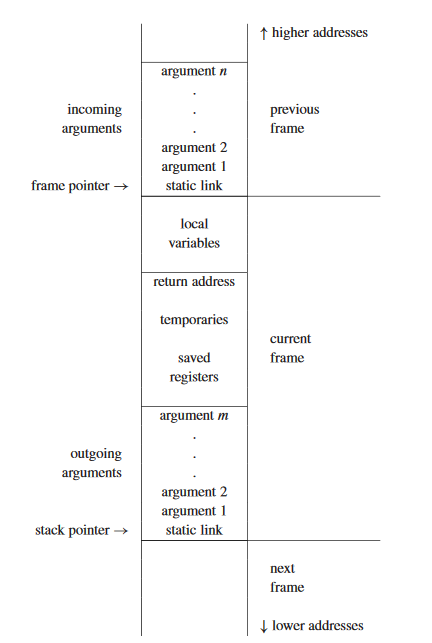
\includegraphics[width=\textwidth]{frame_layout}
	\caption{Een stack frame.}
	\label{fig:stack_frame}
\end{figure}



\subsection{Static Link}

De stack kan ook argumenten bevatten die meegegeven worden aan de functie. Een static link is vooral belangrijk bij geneste en recursieve functies. In program 6.3 (slide 6) moet de variabele \texttt{output} in elke frame beschikbaar zijn. De static link bevat een pointer naar de buitenste functie, zodat deze variabele in elke geneste functie beschikbaar is.



\subsection{Escapes}
Een variable \textit{escapet} uit een stack frame als:
\begin{itemize}
	\item hij passed-by-reference wordt.
	\item of zijn adres genomen wordt.
	\item of hij geaccessed wordt vanuit een geneste functie.
\end{itemize}

Een veranderlijke is \textit{memory-resident} (op de stack plaatsen) als
\begin{itemize}
	\item hij escapet
	\item of niet in een register past
	\item of een array is
	\item of er geen vrij register is
\end{itemize}

Welke parameters moeten op de stack frame zitten en welke niet? Stel volgende functie:
\begin{lstlisting}
int f(int x, int y){
  f(x);
  g(&x);
  return x + y;
}
\end{lstlisting}
Als de functieoproepen $f$ en $g$ er niet zijn, dan moeten $x$ en $y$ niet op de stack. Bij de functie $f$ hangt het af of dat $f$ de parameter aanpast. Bij de functie $g$ moet $x$ zeker in het geheugen zitten en zal dus niet op de stack komen.
\begin{lstlisting}
int f(int x, int y){
  p = &x;
}
\end{lstlisting}


\section{Frames in de Tiger compiler}
\subsection{Frame Interface}
Er is een abstracte representatie nodig van een frame want deze hangt af van de architectuur. Deze komt in \texttt{frame.h}.

\begin{itemize}
	\item \texttt{F\_frame}: datastructuur die een frame voorstelt. 
	\item \texttt{F\_access}: datastructuur die specifieert hoe lokale variabelen moeten geaccesseerd worden (register of geheugen).
	\item \texttt{F\_accessList}: Lijst van \texttt{F\_access} structuren.
	\item \texttt{newFrame(Temp\_label name, U\_boolList formals)}: formals bevat booleans die voor elke parameter aangeeft of hij deze escapet moet worden of niet.
	\item \texttt{allocLocal(F\_frame f, bool escape)}: maakt plaats voor nieuwe veranderlijke in frame $f$, en eventueel is deze escapet.
\end{itemize}

Voorbeeld:
\begin{lstlisting}
F_Frame frame = F_frame(g, U_BoolList(TRUE,
                              U_BoolList(FALSE,
                                 U_BoolList(FALSE,NULL))))
\end{lstlisting}
 
\subsection{Creatie en initialisatie van frames}
\begin{figure}
	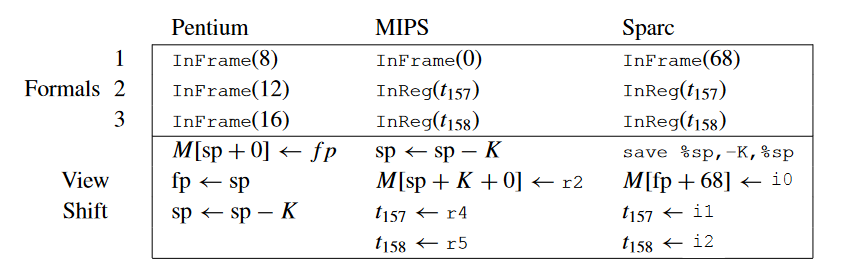
\includegraphics[width=\textwidth]{create_frames}
	\caption{Formele parameters voor $g(x_1, x_2, x_3)$ waarbij $x_1$ escapes.}
	\label{fig:create_frames}
\end{figure}

Bij Pentium moet alles op de stack. In MIPS wordt standaard de eerste 3 argumenten in registers gestoken, maar $x_1$ escapet dus wordt toch in de stack gestoken. 
 
 \subsection{Escapes berekenen}
 Een variable \textit{escapet} uit een stack frame als:
 \begin{itemize}
 	\item hij passed-by-reference wordt.
 	\item of zijn adres genomen wordt.
 	\item of hij geaccessed wordt vanuit een geneste functie.
 \end{itemize}
 Pass-by-reference of het nemen van een referentie is direct zichtbaar in de Abstract Syntax Tree. Om na te gaan of hij geaccessed wordt vanuit een geneste functie wordt de Abstract Syntax Tree recursief overlopen met een symbooltabel (omgeving), maar hier zijn alle veranderlijken gebonden aan booleans: escapes of niet. Deze stap wordt voor semantische analyse en na parsing gedaan. Dus tussen deze twee stappen worden de escapes berekent. Het kan ook efficiënter, maar zien we niet in deze cursus.
 
\subsection{Temporaries en Labels}
\begin{itemize}
	\item Een \textbf{temporary} is een waarde die tijdelijk in een nog te bepalen register wordt bewaard.
	\item Een \textbf{label} is een nog onbekend adres waarde code of statisch gealloceerde data zal terecht komen. Bijvoorbeeld \texttt{string = \textquotedblright een string\textquotedblright} wordt statisch gealloceerd.
	\item Er is ook een aparte interface \texttt{temp.h}.
\end{itemize} 
